\documentclass[•]{article}
\usepackage{graphicx}


\begin{document}
\title{Heat and Mass Week 1}
\maketitle
\section*{Terminology}
\begin{itemize}
\item Convection – Surface effect, reliant on surface area between the two materials, involves one material transferring kinetic energy via some medium. Fluid/gas, gas/solid, fluid/solid.
\item Radiation – Surface effect, majority of energy in infrared spectrum, infrared frequency based on frequency of vibrating atoms, hence thermal radiation based on temperature, higher temperature involves higher frequency of thermal vibrations, higher frequency of infrared radiation.
\item Conduction – How the heat is transferred through a single substance, how heat is transferred through a potato.
\end{itemize}


\section*{Conduction Equations}
Heat conduction can be modelled based on the shape of the object, three prime classifications
\begin{itemize}
\item Rectangular – Expressed as x, y, z and time(t)
\item Cylindrical – Expressed as r, $\theta$, z, and time(t)
\item Spherical – Expressed as r, $\theta$, $\alpha$ and time(t)
\end{itemize}

\section*{Steady versus Transient Heat Transfer}
Two types of thermal system classification, Transient effects are time dependent, while steady effects are time independent. \textbf{Lumped Systems} refer to systems where the temperature is exclusively dependent on time, and has no position dependence.

\section*{One Dimensional Heat Conduction}
One dimensional heat conduction can be modelled using \textbf{Fourier's Law of Heat Conduction} and is as follows:

\begin{equation}
\dot{Q_X} = -kA_X\frac{\partial T}{\partial X}
\end{equation}

This function applies to x, y and z dimensions, ie:

\begin{equation}
\dot{Q_Y} = -kA_Y\frac{\partial T}{\partial Y}
\end{equation}

These can be summed to get the total amount of heat flow at any given time.


\begin{equation}
\dot{Q_n} = \dot{Q_Y} + \dot{Q_X} + \dot{Q_Z}
\end{equation}

\section*{Solving One Dimensional Conduction Problems}
\textbf{Assumptions}: Energy balance of the system

\begin{equation}
\dot{E_Q} + \dot{E_i} - \dot{E_O} = \frac{\partial E}{\partial t}
\end{equation}
Each of the energy terms can be derived using the conduction equations - (3), for example:
\begin{equation}
\dot{E_{in}} - \dot{E_{out}} = \dot{Q_x}
\end{equation}
The energy of the system can be modelled as:

\begin{equation}
\frac{\partial E}{\partial t} = \rho VC_p\frac{\partial T}{\partial t} = \rho\int A_x C_p \frac{\partial T}{\partial t}dx
\end{equation}
Where $C_p$ is a material expression of the heat capacity per unit mass.\\
Equations (5) and (6) can be substituted into equation (4):
\begin{equation}
-kA_x\frac{\partial T}{\partial x} + {\dot{Egen}} = \rho\int A_x C_p \frac{\partial T}{\partial t}dx
\end{equation}
Which can be further manipulated by taking the derivative of both sides w.r.t x. This requires $\rho$ to be constant w.r.t x.

\begin{equation}
\frac{-1}{A_x}\frac{\partial}{\partial x} \Big(-kA_x\frac{\partial T}{\partial x}\Big) + \frac{1}{A_x}\frac{\partial}{\partial x}{\dot{Egen}} = \rho C_p \frac{\partial T}{\partial t}
\end{equation}

If the system is stable with respect to certain variables, it becomes easy to see the relationship between certain elements. For instance, if the system is time invariant, then the time derivative terms dissapear.

\begin{equation}
\frac{-1}{A_x}\frac{\partial}{\partial x} \Big(-kA_x\frac{\partial T}{\partial x}\Big) + \frac{1}{A_x}\frac{\partial}{\partial x}{\dot{Egen}} = 0
\end{equation}

This can be further reduced, and $\dot{E_{gen}}$ can be reduced to instead express the energy per unit area, this variable is represented as: $\dot{e_{gen}}$.

\begin{equation}
\frac{1}{A_x}\frac{\partial}{\partial x} \Big(-kA_x\frac{\partial T}{\partial x}\Big) = \dot{e_{gen}}
\end{equation}

If it can be assumed that $A_x$ is invariant w.r.t, then it can also be removed from the equation.

\begin{equation}
-\frac{\partial^2 T}{{\partial x}^2} = \frac{\dot{e_{gen}}}{k}
\end{equation}

A similar approach can be used to find the solution in which there is no energy generation, and further get the transients in that scenario.\\

Using the assumption that the energy introduced to the system is 0, as well as that the Area is constant w.r.t x the system can be reduced to.
\begin{equation}
\frac{\partial^2 T}{{\partial x}^2} = \rho C_p\frac{\partial T}{\partial t}
\end{equation}

The variable x can be substituted for radius(r) or length(y) or depth(z), and depending on the shape of the material in question, the new equations for Area(A) and so forth can be substituted into the equation 7.

\section*{Temperature Difference Through a Rod}
Solving temperature difference from one end of an insulated rod to another. The area around the rod is insulated. Temperatures are known at x = 0, \& x = L.\\
\subsection*{Scenario 1: $\dot{e_{gen}}$ is 0}
Using equation 11 and using the following assumptions.
\begin{itemize}
\item k is constant w.r.t x
\item $\rho$ is constant w.r.t x
\item System is at Steady state
\item No energy introduced to the system
\item Cross sectional area is constant w.r.t x
\end{itemize}

The equation yields:
\begin{equation}
\frac{\partial^2 T}{{\partial x}^2} = 0
\end{equation}

Which is a seperable differential equation, and can be integrated twice to yield the following equation for temperature with respect to x.

\begin{equation}
T(x) = C_0x + C_1
\end{equation}

The constants can be found by applying the temperature at the known boundary conditions, x = L and x = 0.\\

This can then be used to find the heat flux, $\dot{Q_x}$ through the system. Equation 13 can be substituted into it to find the heat flux.

\begin{equation}
\dot{Q_x} = -kA_x\frac{\partial T}{\partial x} = -kA_xC_0
\end{equation}

\subsection*{Scenario 2: $\dot{e_{gen}}$ is not 0}
The exact same procedure can be repeated in the event that there is energy being generated in the rod. Equation 11 is a seperable differential equation and can thus be integrated twice.

\begin{equation}
T(x) = \frac{-\dot{e_{gen}}}{2k}x^2 + C_0x + C_1
\end{equation}

The heat flux can be found in exactly the same method as before.
\begin{equation}
\dot{Q_x} = -kA_x\frac{\partial T}{\partial x} = -kA_x{\Big(\frac{-\dot{e_{gen}}}{k}x+C_0\Big)}
\end{equation}

\subsection*{Scenario 3: Insulated end}
A different scenario is one in which one end of the rod is insulated, and there is energy being generated within the rod. Assume that the end of the rod that is insulated is at x = L\\

The system again begins with the governing equations, and the system can be solved in exactly the same way as in scenario 2. 

\begin{equation}
T(x) = \frac{-\dot{e_{gen}}}{2k}x^2 + C_0x + C_1
\end{equation}

As well as the heat flux equation

\begin{equation}
\dot{Q(x)} = -kA_x\frac{\partial T}{\partial x} = -kA_x{\Big(\frac{-\dot{e_{gen}}}{k}x+C_0\Big)}
\end{equation}

However, instead of knowing the temperature at both boundaries, we know the temperature at one boundary, and the heat flux at another. This makes solving the constants in the system slightly more complicated, however it should still be straightforward.

\begin{equation}
T(0) = C_1
\end{equation}

\begin{equation}
Q(L) = -kA_x\Big(\frac{-\dot{e_{gen}}}{k}L+C_0\Big)
\end{equation}

\begin{equation}
T(L) = \frac{-\dot{e_{gen}}}{2k}L^2 + C_0L + C_1
\end{equation}

\section*{Convection Equation}
Heat Convection is proportional to the temperature drop between the two mediums.

\begin{equation}
\dot{Q} = h_sA_s(T_s - T_{\infty})
\end{equation}

\subsection*{Problem 1}
A heater is delivering heat to one end of an insulated rod, the other end is exposed to air.\\

The problem can be solved by using the energy flowing into the system at one side of the system, and solving for the energy out at the other side of the system. The heat flux at one end of the system can be known, due to the presense of the heater.

\begin{equation}
\dot{Q} = P_{htr} = -kA_x\frac{dT}{dX}
\end{equation}

Due to the fact that there is no energy introduced in the rod, the temperature difference through the rod is a linear drop, hence there is a constant Q through the rod, this can be used to get the expression for one of the coefficients.

\begin{equation}
\frac{dT}{dx} = C_0 = \frac{-P_{htr}}{kA_x}
\end{equation}

Which can be substitued into the solution for the temperature as a function of x.
\begin{equation}
T(x) = \frac{-P_{htr}}{kA_x}x + C_1
\end{equation}

As the heat flux through the system is constant, the convection equation can be used to compute the temperature at the other end.

\begin{equation}
\dot{Q} = h_sA_s(T_s - T_{\infty}) = P_{htr}
\end{equation}

As $T_{\infty}$ is known, the temperature at the surface can be known. This allows for the coefficient to be found at the boundary.

\section*{Radiation}
The procedure for radiation is identical to convection, however the equation for radiation is:

\begin{equation}
\dot{Q} = \epsilon\sigma(T_s^4 - T_{\infty}^4)
\end{equation}

\section*{Interface Between Materials}
The interface between two materials can be dealt with by setting the temperature and heat flux at the interface equal.

\section*{Heat Generation in a Solid}
The temperature profile in a solid with uniform energy generation should be computed using the standard equation from week 1.

\subsection*{Example}
Temperature profile in an insulated rod, with both ends exposed to the same temperature.

\section*{Heat Conductivity and Temperature}
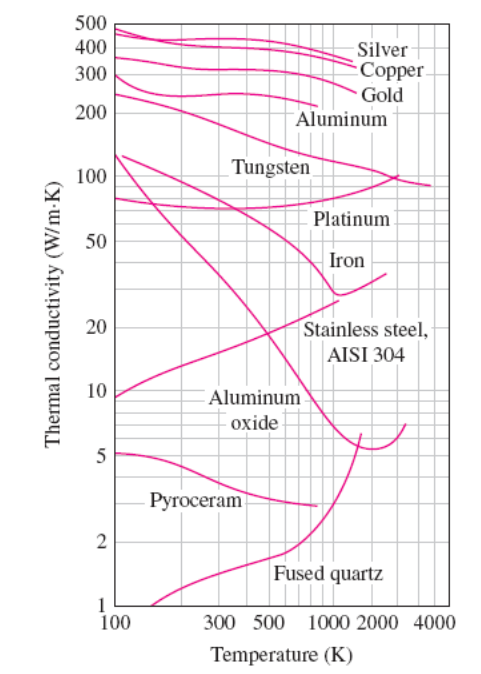
\includegraphics[scale=0.5]{condCurve}

\end{document}